\section{Практична частина}
\setlength{\parindent}{4em}
\begin{center}
  {\textbf{\emph{Метод Бесселя}}}
\end{center}
Робоча формула:
$$f' = \frac{SS'}{S-S'} = \frac{L^2 - l^2}{4L}$$
\begin{figure}[ht]

\centering

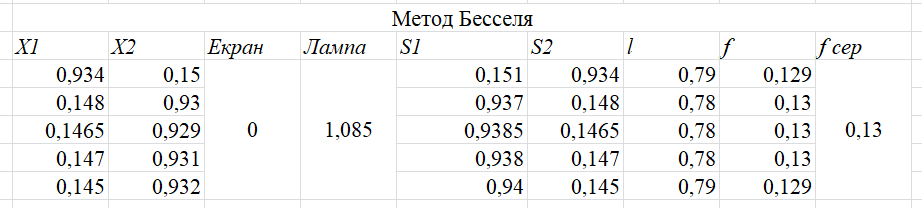
\includegraphics[width=0.55\linewidth]{Pic/Prac1.png}

\caption{Отримані результати}

\label{Prac1}

\end{figure}
\begin{center}
  {\textbf{\emph{Метод Аббе}}}
\end{center}
Робоча формула:
$$f=-f'=\frac{\Delta y_1' y_2'}{y(y_2'-y_1')}$$
\begin{figure}[ht]

\centering

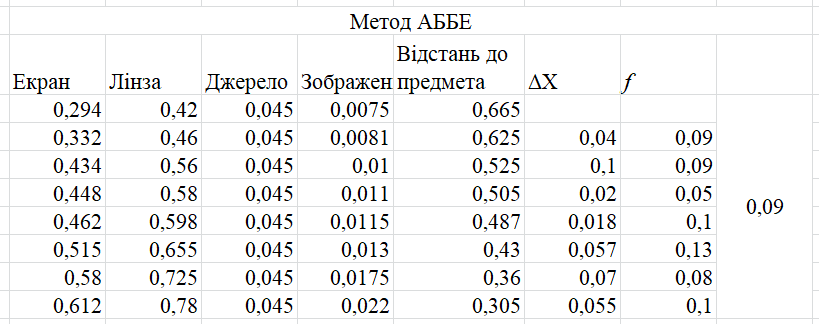
\includegraphics[width=0.55\linewidth]{Pic/Prac2.png}

\caption{Отримані результати}

\label{Prac2}

\end{figure}
\begin{center}
  {\textbf{\emph{Знаходження фокусної відстані лінзи за допомогою труби}}}
\end{center}
\begin{figure}[ht]

\centering

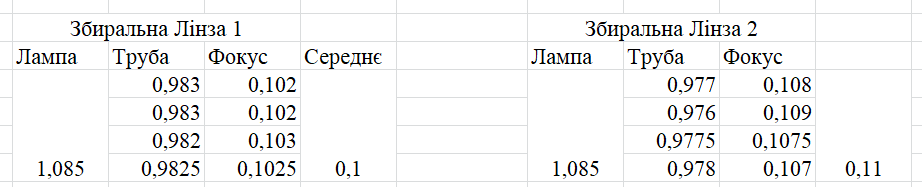
\includegraphics[width=0.6\linewidth]{Pic/Prac3.png}

\caption{Отримані результати}

\label{Prac3}

\end{figure}

\newpage
\begin{center}
  {\textbf{\emph{Знаходження фокусної відстані лінзи за формулою тонкої лінзи}}}
\end{center}
Робочі формули:
$$\frac{1}{F} = \frac{1}{f}+\frac{1}{d}$$
$$-\frac{1}{F} = -\frac{1}{d}+\frac{1}{f}$$
\begin{figure}[ht]

\centering

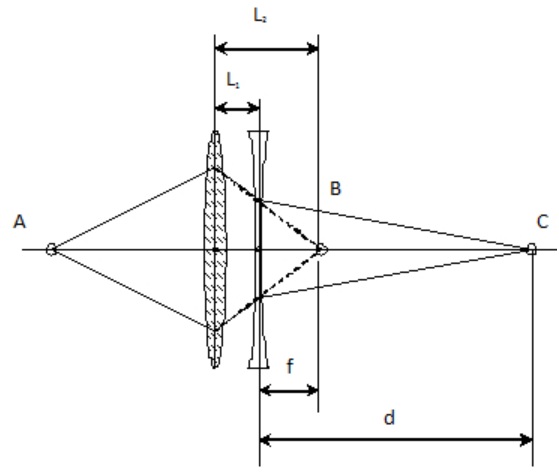
\includegraphics[width=0.6\linewidth]{Pic/Prac5.png}

\caption{Відстані для розсіювальної лінзи}

\label{Prac5}

\end{figure}
\begin{figure}[ht]

\centering

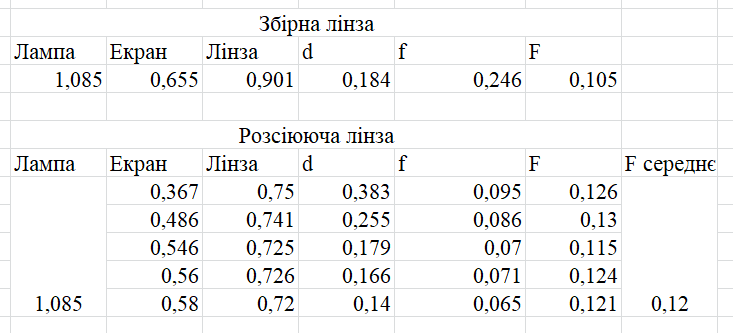
\includegraphics[width=0.6\linewidth]{Pic/Prac4.png}

\caption{Отримані результати}

\label{Prac4}

\end{figure}
\newpage
\subsection{Отримані результати для фокусної відстані збиральної лінзи:}

\begin{enumerate}
  \item $F=0,09 m$
  \item $F=0,105m$
  \item $F=0,105m$
\end{enumerate}
Отримані результати для фокусної відстані розсіювальної лінзи:
\begin{enumerate}
  \item $F=0,13 m$
  \item $F=0,12m$
\end{enumerate}
